% CVPR 2022 Paper Template
% based on the CVPR template provided by Ming-Ming Cheng (https://github.com/MCG-NKU/CVPR_Template)
% modified and extended by Stefan Roth (stefan.roth@NOSPAMtu-darmstadt.de)

\documentclass[10pt,twocolumn,letterpaper]{article}

%%%%%%%%% PAPER TYPE  - PLEASE UPDATE FOR FINAL VERSION
%\usepackage[review]{cvpr}      % To produce the REVIEW version
\usepackage{cvpr}              % To produce the CAMERA-READY version
%\usepackage[pagenumbers]{cvpr} % To force page numbers, e.g. for an arXiv version

% Include other packages here, before hyperref.
\usepackage{graphicx}
\usepackage{amsmath}
\usepackage{amssymb}
\usepackage{booktabs}
\usepackage{tikz}
\usetikzlibrary{shapes.geometric, arrows.meta, positioning, fit, backgrounds}

\newcommand{\latex}{\LaTeX\xspace}
\newcommand{\tex}{\TeX\xspace}


% It is strongly recommended to use hyperref, especially for the review version.
% hyperref with option pagebackref eases the reviewers' job.
% Please disable hyperref *only* if you encounter grave issues, e.g. with the
% file validation for the camera-ready version.
%
% If you comment hyperref and then uncomment it, you should delete
% ReviewTempalte.aux before re-running LaTeX.
% (Or just hit 'q' on the first LaTeX run, let it finish, and you
%  should be clear).
\usepackage[pagebackref,breaklinks,colorlinks]{hyperref}


% Support for easy cross-referencing
\usepackage[capitalize]{cleveref}
\crefname{section}{Sec.}{Secs.}
\Crefname{section}{Section}{Sections}
\Crefname{table}{Table}{Tables}
\crefname{table}{Tab.}{Tabs.}

\begin{document}

%%%%%%%%% TÍTULO

\title{Detección y Clasificación de Patógenos Foliares mediante Visión por Computador}

\author{
   Gabriel Sánchez Muñoz\\{\tt\small gabrielfsm@correo.ugr.es}
   \and
   Germán Rodríguez Vidal\\{\tt\small germanrv@correo.ugr.es}
   \and
   Pablo García Bas\\{\tt\small pablogarciabas@correo.ugr.es}
   \and
   Miguel Ángel Moreno Castro\\{\tt\small miguelangelmc@correo.ugr.es}
}

\maketitle

%%%%%%%%% RESUMEN
\begin{abstract}
   La detección temprana y precisa de enfermedades vegetales es crítica para la agricultura de precisión y la seguridad alimentaria.
   Los enfoques actuales basados en \textit{Deep Learning}, a pesar de mostrar resultados prometedores, suelen carecer de información contextual sobre el huésped, lo que limita su precisión en escenarios de múltiples cultivos. 
   Este trabajo propone un enfoque jerárquico de dos etapas para abordar esta limitación. En primer lugar, se realiza una clasificación de la especie arbórea para establecer un contexto biológico y, posteriormente, un detector de objetos localiza y clasifica los patógenos específicos asociados a dicha especie.
   Los resultados muestran que incorporar la identificación previa del huésped incrementa la precisión media (mAP) en un 10\% respecto a los detectores genéricos de una sola etapa (\textit{"end-to-end"}), demostrando la superioridad de los modelos condicionados biológicamente.
\end{abstract}

%%%%%%%%% CUERPO DEL TEXTO
\section{Introducción}
\label{sec:intro}
Las enfermedades de las plantas representan una amenaza significativa para la seguridad alimentaria y la estabilidad económica agrícola, causando pérdidas estimadas de hasta el 30\% en el rendimiento de los cultivos cada año \cite{savary2019global}. 
La identificación temprana y precisa de estas patologías es crucial para aplicar medidas de control eficaces y minimizar el uso de químicos. 
Tradicionalmente, este diagnóstico ha dependido de la inspección visual manual por parte de expertos, un proceso que resulta laborioso, subjetivo y difícil de escalar a grandes explotaciones \cite{barbedo2013digital}.

En la última década, la visión por computador y, específicamente, el aprendizaje profundo, han emergido como herramientas poderosas para automatizar esta tarea. 
El uso de Redes Neuronales Convolucionales (\textit{CNNs}) ha permitido grandes avances tanto en la clasificación de imágenes (identificar si una hoja está enferma) como en la detección de objetos (localizar la lesión exacta en la hoja) \cite{mohanty2016using}. 
Sin embargo, la mayoría de las arquitecturas actuales abordan la detección de enfermedades como un problema monolítico donde los modelos se entrenan para detectar cualquier enfermedad en cualquier tipo de hoja simultáneamente, ignorando a menudo la estructura jerárquica natural de la taxonomía biológica.

Debido a que muchas patologías foliares comparten características visuales similares, independientemente de la especie, los detectores agnósticos al huésped sufren de una alta confusión inter-clase. 
Esto suele derivar en predicciones erróneas donde se asocian enfermedades a plantas incompatibles, reduciendo la precisión y confiabilidad del sistema en aplicaciones del mundo real.

Para resolver esto, proponemos un enfoque jerárquico que imita el diagnóstico experto donde primero se identifica la especie del árbol para simplificar la búsqueda de la enfermedad y luego se aplica un detector especializado para esa especie.

\section{Estado del Arte}

\subsection{Clasificación}

Los dos paradigmas principales en clasificación de imágenes son las arquitecturas basadas en \textit{Vision Transformers} (\textit{ViT}) y las Redes Neuronales Convolucionales (\textit{CNNs}). 
Nuestro objetivo fue contrastar la capacidad de modelado global de los \textit{Transformers} frente a la eficiencia inductiva de las \textit{CNNs}. 
Adicionalmente, dada la orientación práctica de este proyecto hacia una futura aplicación móvil, se incluyó en el estudio un modelo diseñado específicamente para entornos de recursos limitados (\textit{edge devices}).

\subsubsection{MaxViT}

Dentro de la familia de los \textit{Transformers}, \textit{MaxViT} (\textit{Multi-Axis Vision Transformer}) combina tanto mecanismos de atención global como convoluciones locales para capturar características a múltiples escalas \cite{tu2022maxvit}.
Su característica distintiva es el mecanismo de \textit{Multi-Axis Self-Attention} (\textit{Max-SA}), que descompone el cálculo de atención en dos operaciones; atención local (\textit{Block Attention}) para capturar texturas finas, y atención global dispersa (\textit{Grid Attention}) para relacionar partes distantes de la imagen.

\subsubsection{EfficientNetV2}

\textit{EfficientNetV2} es una evolución de la familia de \textit{EfficientNet} (\textit{CNN}) que optimiza tanto la arquitectura como el proceso de entrenamiento para mejorar la velocidad y precisión \cite{tan2021efficientnetv2}.
Esta arquitectura mejora a su predecesora mediante la introducción de bloques \textit{Fused-MBConv} \cite{tan2021efficientnetv2}.
Estos bloques reemplazan las convoluciones \textit{depthwise} separables tradicionales por convoluciones estándar $3 \times 3$ fusionadas en las primeras capas.

\subsubsection{MobileNet}

\textit{MobileNet} es una arquitectura basada en \textit{CNN} diseñada para dispositivos móviles y aplicaciones de \textit{edge computing} \cite{howard2017mobilenets}.
La base de su eficiencia radica en las convoluciones \textit{depthwise} separables, que factorizan la operación de convolución estándar en dos capas más ligeras (de tamaños $3 \times 3$ y $1 \times 1$), reduciendo drásticamente la cantidad de parámetros y operaciones \cite{howard2017mobilenets}. 
Aunque su capacidad de representación es menor que los modelos anteriores, su inclusión es crítica para evaluar el \textit{trade-off} entre precisión y latencia en una aplicación real para agricultores.

\subsection{Detección de Objetos}

El objetivo fundamental en detección de objetos es localizar y clasificar regiones de interés (\textit{bounding boxes}). 
Históricamente, métodos dominantes como \textit{Deformable Parts Model} (\textit{DPM}) abordaban este problema mediante un enfoque de ventana deslizante (\textit{sliding window}) que resultaban inviables computacionalmente al procesar todas las posibles sub-ventanas \cite{felzenszwalb2010dpm}.

La evolución comenzó con \textbf{R-CNN}, un modelo de 3 etapas donde una búsqueda selectiva genera regiones potencialmente interesantes, una \textit{CNN} extrae características y un \textit{SVM} las clasifica \cite{girshick2014rcnn}. 
Sus limitaciones principales son el alto coste de procesar regiones por separado y la falta de aprendizaje en la búsqueda selectiva. 

\subsubsection{Faster R-CNN}

\textit{Faster R-CNN} integra la propuesta de regiones dentro de la red neuronal, reemplazando el algoritmo fijo por una \textit{Region Proposal Network} (\textit{RPN}) entrenable y más rápida \cite{ren2016fasterrcnn}. 

En primer lugar se definen \textit{anchor points} sobre el mapa de características de la imagen, actuando como centros de posibles regiones con diferentes escalas y \textit{ratios}. Seguidamente, la \textit{RPN} predice simultáneamente la probabilidad de objeto y las coordenadas del \textit{bounding box}.

A pesar de su alta precisión, el hecho de ser un modelo de dos etapas penaliza su velocidad de inferencia.
\subsubsection{YOLO}

Como respuesta a la latencia, \textit{You Only Look Once} (\textit{YOLO}) redefinió la detección no como una clasificación de regiones, sino como un problema único de regresión, descartando por completo el \textit{pipeline} disjunto de \textit{DPM} y \textit{R-CNN}.

\textit{YOLO} utiliza una única red neuronal convolucional que procesa la imagen completa de una sola vez.
Divide la imagen en una cuadrícula ($S \times S$) donde cada celda predice $B$ \textit{bounding boxes} y sus respectivas puntuaciones de confianza.

La arquitectura unificada de \textit{YOLO} permite una inferencia en tiempo real inalcanzable para los métodos de dos etapas \cite{redmon2016yolo}. Mientras que \textit{Faster R-CNN} procesa aproximadamente 0.5 \textit{FPS}, \textit{YOLO} alcanza los 45 \textit{FPS}, ofreciendo la inmediatez necesaria para aplicaciones agrícolas prácticas.

\section{Metodología Propuesta}

\subsection{Dataset}

Para validar nuestro enfoque jerárquico, hemos confeccionado un \textit{dataset} que integra imágenes de tres cultivos. 
Las imágenes provienen de la plataforma \textit{Roboflow Universe}, que contiene una gran cantidad de \textit{datasets} de código abierto, y han sido seleccionadas por su calidad y variedad de condiciones de iluminación.

\begin{itemize}
   \item \textit{Rose Dataset}: Consta de 2,725 imágenes y abarca 4 clases (\textit{Black Spot}, \textit{Downy Mildew}, \textit{Powdery Mildew} y \textit{Healthy}).
   \item \textit{Potato Dataset}: Comprende 812 imágenes distribuidas en 3 clases (\textit{Early Blight}, \textit{Late Blight}, \textit{Healthy}).
   \item \textit{Apple Dataset}: Incluye 1582 imágenes que cubren 5 clases (\textit{Alternaria Spot}, \textit{Brown Spot}, \textit{Gray Spot}, \textit{Rust}, \textit{Healthy}).
\end{itemize}

El \textit{dataset} combinado se dividió aleatoriamente en subconjuntos de Entrenamiento (70\%), Validación (15\%) y Prueba (15\%), preservando la estratificación de clases para garantizar una evaluación equilibrada.

El \textit{dataset} de manzanas requirió un preprocesamiento adicional, ya que sus anotaciones originales estaban en formato de máscaras de segmentación semántica en lugar de coordenadas de \textit{bounding boxes}. 
Utilizando \textit{OpenCV} (\texttt{cv2.findContours} y \texttt{cv2.boundingRect}), se convirtieron automáticamente las máscaras de las lesiones en \textit{bounding boxes}, generando las coordenadas necesarias para su integración en el flujo de trabajo de \textit{YOLO}.
\begin{figure*}[t] % El asterisco hace que ocupe el ancho de las dos columnas
\centering
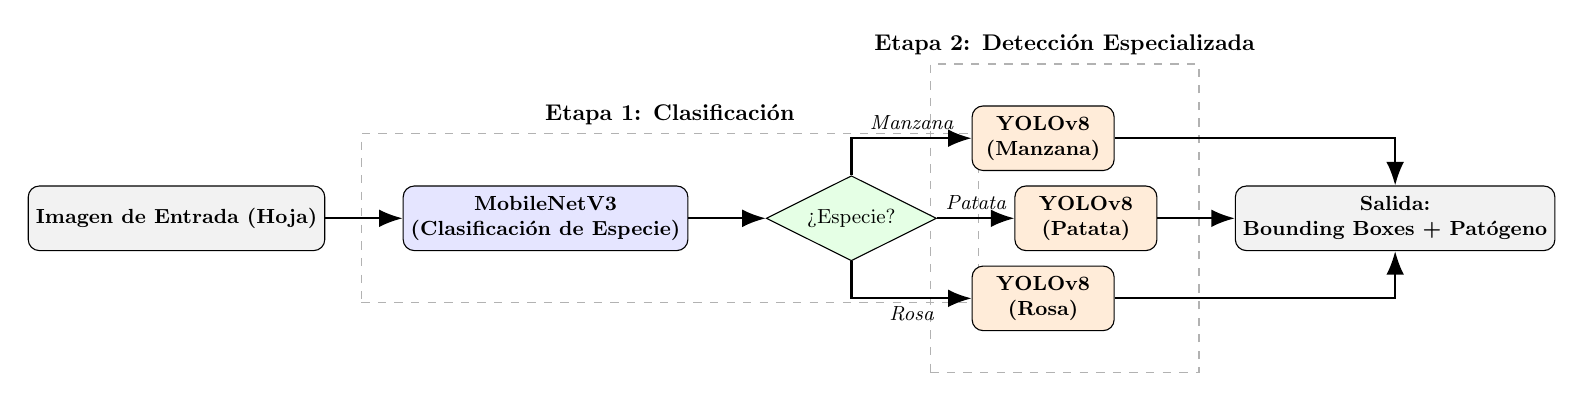
\begin{tikzpicture}[
    scale=0.82, transform shape,
    node distance=1.2cm and 1.2cm,
    box/.style={draw, rectangle, rounded corners, minimum width=2.8cm, minimum height=1cm, text centered, align=center, font=\bfseries\small, fill=blue!10},
    yolo/.style={draw, rectangle, rounded corners, minimum width=2.2cm, minimum height=1cm, text centered, align=center, font=\bfseries\small, fill=orange!15},
    decision/.style={draw, diamond, aspect=2, minimum width=2.2cm, minimum height=1cm, text centered, align=center, font=\small, fill=green!10},
    arrow/.style={-{Latex[length=3mm]}, thick},
    label_text/.style={font=\small\itshape}
]

% Nodos principales
\node (input) [box, fill=gray!10] {Imagen de Entrada (Hoja)};

% Etapa 1: Clasificación
\node (mobilenet) [box, right=of input] {MobileNetV3\\(Clasificación de Especie)};

% Decisión
\node (switch) [decision, right=of mobilenet] {¿Especie?};

% Etapa 2: Detección (YOLOv8)
\node (yolo_apple) [yolo, above right=0.4cm and 1.2cm of switch] {YOLOv8\\(Manzana)};
\node (yolo_potato) [yolo, right=1.2cm of switch] {YOLOv8\\(Patata)};
\node (yolo_rose) [yolo, below right=0.4cm and 1.2cm of switch] {YOLOv8\\(Rosa)};

% Salida
\node (output) [box, fill=gray!10, right=of yolo_potato] {Salida:\\Bounding Boxes + Patógeno};

% Conexiones
\draw [arrow] (input) -- (mobilenet);
\draw [arrow] (mobilenet) -- (switch);

% Flechas del switch a los YOLOs
\draw [arrow] (switch.north) |- (yolo_apple.west) node[pos=0.75, above, label_text] {Manzana};
\draw [arrow] (switch.east) -- (yolo_potato.west) node[midway, above, label_text] {Patata};
\draw [arrow] (switch.south) |- (yolo_rose.west) node[pos=0.75, below, label_text] {Rosa};

% Flechas de los YOLOs a la salida
\draw [arrow] (yolo_apple.east) -| (output.north);
\draw [arrow] (yolo_potato.east) -- (output.west);
\draw [arrow] (yolo_rose.east) -| (output.south);

% Recuadro de fondo (opcional para agrupar las etapas)
\begin{scope}[on background layer]
    \node [draw=black!30, dashed, fit=(mobilenet) (switch), inner sep=15pt, label=above:{\textbf{Etapa 1: Clasificación}}] {};
    \node [draw=black!30, dashed, fit=(yolo_apple) (yolo_potato) (yolo_rose), inner sep=15pt, label=above:{\textbf{Etapa 2: Detección Especializada}}] {};
\end{scope}

\end{tikzpicture}
\caption{Arquitectura del Pipeline Especializado}
\label{fig:pipeline}
\end{figure*}

\subsection{Arquitecturas}

Para evaluar la eficacia del enfoque jerárquico propuesto, se implementaron y compararon tres variantes arquitectónicas del \textit{pipeline} de detección. Todas comparten la etapa inicial de clasificación de especies mediante MobileNet, pero difieren en la estrategia de especialización durante la detección:

\begin{itemize}
    \item \textbf{\textit{Pipeline} Especializado}: La predicción del clasificador actúa como un enrutador dinámico. 
    Como se ilustra en la Figura \ref{fig:pipeline}, dependiendo de la especie identificada, la imagen se procesa con un detector YOLOv8 independiente entrenado exclusivamente con el subconjunto de datos correspondiente (Rosa, Patata o Manzana). Esto maximiza la especialización del modelo y elimina la confusión inter-especie a nivel de detector, alineándose con el diagnóstico experto donde cada patología se evalúa en su contexto biológico específico.
    
    \item \textbf{\textit{Pipeline} Unificado}: El clasificador identifica la especie, pero la detección se realiza mediante un único modelo YOLOv8 global entrenado con el \textit{dataset} combinado de todas las especies y patógenos (Figura \ref{fig:pipeline_single}).
    Sin embargo, la predicción del clasificador se utiliza como mecanismo de \textit{masking} lógico, restringiendo el espacio de búsqueda exclusivamente a las enfermedades biológicamente plausibles para la especie detectada. Este enfoque evalúa si el condicionamiento post-procesado es suficiente para reducir la ambigüedad sin incrementar el coste computacional de múltiples detectores.
    
    \item \textbf{Monolítico}: Un único detector YOLOv8 global entrenado sin información de especie, procesando todas las clases de patógenos simultáneamente en un enfoque completamente agnóstico al huésped. Esta configuración sirve como línea base para cuantificar el impacto de la información contextual biológica en la precisión y la generalización.
\end{itemize}

\section{Experimentos}

\subsection{Selección de Modelos}

La definición de la arquitectura final se fundamentó en un análisis exhaustivo del compromiso entre precisión predictiva y coste computacional, priorizando la viabilidad del despliegue en dispositivos móviles. 

\subsubsection{Clasificación}

Para la etapa de clasificación de especies se seleccionó \textbf{MobileNet} \cite{howard2017mobilenets} tras compararlo con modelos de mayor densidad como MaxViT y EfficientNetV2. 
Los experimentos preliminares revelaron que, dada la baja cardinalidad del problema de clasificación (limitado a tres clases), los modelos de alta capacidad sufrían una saturación de rendimiento, no aportando ganancias significativas de precisión que justificaran la latencia adicional introducida. 

\begin{figure}[h!]
    \centering
    \includegraphics[width=0.45\textwidth]{resources/classification.png}
    \caption{Comparativa de precisión entre modelos de clasificación.}
    \label{fig:classification_comparison}
\end{figure}

Como se observa en las Figuras \ref{fig:classification_comparison} y \ref{fig:inference_time_classification}, MobileNet demostró ofrecer un rendimiento competitivo con una fracción de los parámetros y, crucialmente, una latencia de inferencia significativamente menor que los otros, alineándose con los requisitos de eficiencia del sistema y viabilidad del despliegue en dispositivos móviles.

\begin{figure}[h!]
    \centering
    \includegraphics[width=0.4\textwidth]{resources/classification_inftime.png}
    \caption{Comparativa de latencia de inferencia entre modelos de clasificación.}
    \label{fig:inference_time_classification}
\end{figure}

\subsubsection{Detección de Objetos}
Para la etapa de localización de patógenos, el estudio comparativo descartó inicialmente los detectores de dos etapas como \textbf{Faster R-CNN}. 
A pesar de su teórica precisión, esta arquitectura mostró una tendencia temprana al sobreajuste y una velocidad de inferencia insuficiente para la experiencia de usuario en tiempo real, debido a la sobrecarga computacional de RPN. Por consiguiente, se optó por el paradigma de una sola etapa, acotando la selección final a las variantes \textit{small} de \textbf{YOLOv8} y la reciente \textbf{YOLO11}.

\begin{table}[ht]
\centering

\scalebox{0.9}{
    \begin{tabular}{lccc}
    \toprule
    \textbf{Modelo} & \textbf{Params (M)} & \textbf{mAP@50} & \textbf{mAP@50-95} \\
    \midrule
    \textbf{YOLOv8s}   & 11.2 & \textbf{0.8741} & \textbf{0.5899} \\
    YOLOv11s           & 9.4  & 0.8709          & 0.5856          \\
    YOLOv11n           & \textbf{2.6}  & 0.8652          & 0.5815          \\
    YOLOv8n            & 8.7  & 0.8649          & 0.5797          \\
    YOLOv5s            & 9.1  & 0.8691          & 0.5792          \\
    YOLOv5n            & \textbf{2.6}  & 0.8655          & 0.5775          \\
    YOLOv3-tiny        & 8.7  & 0.8365          & 0.5043          \\
    Faster R-CNN       & $>40$ & 0.7473          & 0.4321          \\
    \bottomrule
    \end{tabular}
}
\caption{Comparativa de eficiencia (Parámetros) y precisión promedio (mAP) incluyendo Faster R-CNN.}
\label{tab:promedio_modelos_simple}
\end{table}

Aunque ambas versiones de YOLO mostraron un desempeño sobresaliente, la balanza se inclinó finalmente a favor de \textbf{YOLOv8s} por su superior estabilidad y eficiencia.
En términos de robustez inter-dominio, la versión 8 ofreció una mayor consistencia, superando a la v11 en el \textit{dataset} de rosas (+1.5\% mAP) y manteniendo un empate técnico en patatas, mientras que las mejoras de la v11 en manzanas fueron marginales y no compensaron su inestabilidad en otros escenarios. 
Críticamente, YOLOv8s demostró ser computacionalmente más eficiente, requiriendo menores tiempos de convergencia durante el entrenamiento y ofreciendo una latencia de inferencia un 6.4\% menor (2.66 img/s frente a 2.50 img/s). 

Esta combinación de estabilidad predictiva y agilidad de procesamiento consolidó a YOLOv8s como el detector idóneo para la arquitectura jerárquica propuesta.

\begin{figure*}[t]
\centering
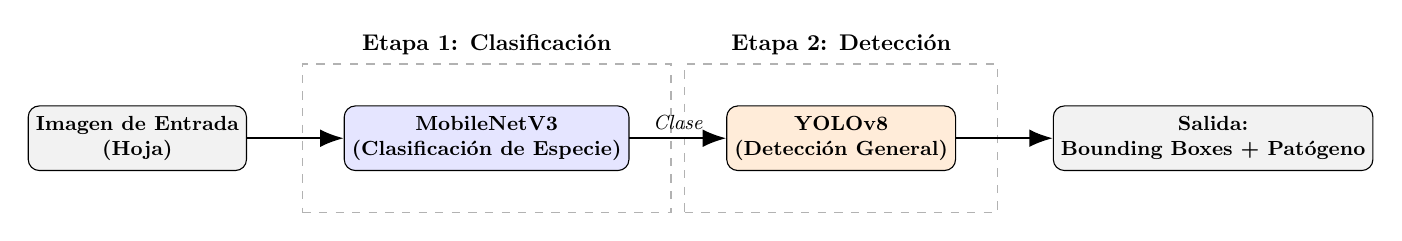
\begin{tikzpicture}[
    scale=0.82, transform shape,
    node distance=1.5cm and 1.5cm, % Aumenté un poco la distancia horizontal para claridad
    box/.style={draw, rectangle, rounded corners, minimum width=2.8cm, minimum height=1cm, text centered, align=center, font=\bfseries\small, fill=blue!10},
    yolo/.style={draw, rectangle, rounded corners, minimum width=2.2cm, minimum height=1cm, text centered, align=center, font=\bfseries\small, fill=orange!15},
    arrow/.style={-{Latex[length=3mm]}, thick},
    label_text/.style={font=\small\itshape, align=center}
]

% --- Nodos Principales ---

% 1. Entrada
\node (input) [box, fill=gray!10] {Imagen de Entrada\\(Hoja)};

% 2. Etapa 1: Clasificación
\node (mobilenet) [box, right=of input] {MobileNetV3\\(Clasificación de Especie)};

% 3. Etapa 2: Detección (Unificada)
% Aquí sustituimos el switch y los 3 YOLOs por uno solo
\node (yolo_unified) [yolo, right=of mobilenet] {YOLOv8\\(Detección General)};

% 4. Salida
\node (output) [box, fill=gray!10, right=of yolo_unified] {Salida:\\Bounding Boxes + Patógeno};

% --- Conexiones ---

% De Entrada a MobileNet
\draw [arrow] (input) -- (mobilenet);

% De MobileNet al YOLO único
% La etiqueta indica que se pasa la información de la especie o el contexto
\draw [arrow] (mobilenet) -- (yolo_unified) node[midway, above, label_text] {Clase};

% Del YOLO a la Salida
\draw [arrow] (yolo_unified) -- (output);

% --- Recuadros de fondo (Etapas) ---
\begin{scope}[on background layer]
    % Etapa 1
    \node [draw=black!30, dashed, fit=(mobilenet), inner sep=15pt, label=above:{\textbf{Etapa 1: Clasificación}}] {};
    
    % Etapa 2 (Ahora solo contiene el YOLO unificado)
    \node [draw=black!30, dashed, fit=(yolo_unified), inner sep=15pt, label=above:{\textbf{Etapa 2: Detección}}] {};
\end{scope}

\end{tikzpicture}
\caption{Arquitectura del Pipeline Unificado}
\label{fig:pipeline_single}
\end{figure*}




\subsection{Configuración Experimental}

La ejecución de los experimentos y el entrenamiento de los modelos se llevaron a cabo utilizando el entorno de computación de Google Colab, aprovechando la aceleración por hardware mediante GPUs NVIDIA A100.

Para la etapa inicial de clasificación de especies, se instanció la arquitectura \textbf{MobileNetV3 Small} con pesos pre-entrenados en ImageNet-1k, implementando una estrategia de aprendizaje progresivo en dos fases. 

Inicialmente, se aplicó \textit{freezing} a la red troncal para entrenar exclusivamente la cabecera de clasificación durante 5 épocas, empleando el optimizador AdamW con una tasa de aprendizaje de $1 \times 10^{-3}$. 
Posteriormente, se procedió al \textit{unfreezing} de los parámetros para una fase de \textit{fine-tuning} durante 10 épocas, donde el \textit{learning rate} se redujo a $8 \times 10^{-6}$. 

En lo referente a la etapa de detección, la configuración del modelo \textbf{YOLOv8s} también se fundamentó en \textit{transfer learning} desde el \textit{dataset} COCO. 
El entrenamiento se estandarizó con una resolución de entrada de $640 \times 640$ píxeles y un \textit{batch size} de 16, extendiéndose a lo largo de 30 épocas completas.
Este proceso mantuvo las configuraciones de optimización predeterminadas del \textit{framework} Ultralytics \cite{jocher2023ultralytics} e integró técnicas de \textit{data augmentation} en tiempo de ejecución, destacando el uso de \textit{mosaic augmentation}, para incrementar la variabilidad de las muestras y mejorar la capacidad de generalización del modelo.

\subsection{Métricas de Evaluación}

En tareas de detección de objetos, la métrica estándar es la \textit{mean average precision} (mAP), la cual se fundamenta en el coeficiente de \textit{Intersection over Union} (IoU).

\begin{equation}
    \text{IoU} = \frac{|B_p \cap B_{gt}|}{|B_p \cup B_{gt}|}
\end{equation}

La IoU cuantifica la superposición entre la predicción del modelo ($B_p$) y la anotación real ($B_{gt}$) de la \textit{bounding box}, sirviendo como criterio para determinar el éxito de una detección.

En la práctica se reportan los valores de \textbf{mAP50} y \textbf{mAP50-95} para ofrecer una visión completa del desempeño del detector. 
El \textbf{mAP50} establece un umbral de tolerancia relajado ($\text{IoU} \geq 0.50$), considerando válida cualquier predicción que se solape al menos en un 50\% con la referencia real, lo cual es indicativo de la capacidad del modelo para una localización general del objeto. 
Por el contrario, la métrica \textbf{mAP50-95} es mucho más exigente, ya que calcula el promedio de la precisión sobre diez umbrales progresivos de IoU (desde 0.50 hasta 0.95 en intervalos de 0.05).

\begin{table*}[!t]
\centering
\scalebox{1}{ 
    \begin{tabular}{lcccccc}
    \toprule
     & \multicolumn{2}{c}{\textbf{Monolítico}} & \multicolumn{2}{c}{\textbf{Unificado}} & \multicolumn{2}{c}{\textbf{Especializado}} \\
    \textbf{Especie} & \textbf{mAP50} & \textbf{mAP50-95} & \textbf{mAP50} & \textbf{mAP50-95} & \textbf{mAP50} & \textbf{mAP50-95} \\
    \midrule
    Manzana & 0.9302 & 0.6932 & 0.9302 & 0.6931 & 0.9530 & 0.7250 \\
    Patatas & 0.7780 & 0.6153 & 0.7780 & 0.6153 & 0.8411 & 0.6654 \\
    Rosas   & 0.9144 & 0.5445 & 0.9142 & 0.5441 & 0.9569 & 0.6490 \\
    \midrule
    \textbf{Avg} & \textbf{0.8742} & \textbf{0.6177} & \textbf{0.8741} & \textbf{0.6175} & \textbf{0.9170} & \textbf{0.6798} \\
    \bottomrule
    \end{tabular}%
}
\caption{Comparativa de rendimiento (mAP50 y mAP50-95) entre las tres estrategias evaluadas.}
\label{tab:resultados_resumen}
\end{table*}

\subsection{Resultados}

Al analizar la Tabla \ref{tab:resultados_resumen}, nos encontramos con un escenario muy interesante. A diferencia de lo que podría esperarse, el modelo \textbf{Monolítico} demostró ser bastante competente, alcanzando un mAP50 promedio de 0.8742. 
Esto indica que la arquitectura YOLOv8 es robusta y capaz de aprender múltiples clases simultáneamente sin desmoronarse. 
Sin embargo, los datos también revelan que este enfoque generalista tiene una cota superior, aunque detecta bien, le cuesta perfeccionar los resultados en las clases más difíciles o cuando se requiere una precisión geométrica muy alta.

La comparación con el método \textbf{Unificado} es reveladora. Los resultados son prácticamente idénticos a los del Monolítico (por ejemplo, en patatas ambos obtienen un 0.7780 y en manzanas un 0.9302).
Esto nos indica que el modelo base no estaba cometiendo errores de confusión de especies, por lo que aplicar un filtro lógico a posteriori no aportó ninguna mejora real.
El problema no era la confusión taxonómica, sino la falta de capacidad de la red para especializarse en los detalles finos de cada plaga cuando tiene que atender a todas a la vez.

Aquí es donde brilla el enfoque \textbf{Especializado} puesto que al entrenar modelos dedicados logramos romper ese techo de rendimiento que limitaba a los otros dos enfoques.
La mejora más notable se dio en la clase patatas, la más difícil del conjunto, donde la precisión saltó de un 0.77 a un 0.84. 
De igual forma, en las rosas, aunque la detección ya era buena, el modelo especializado mejoró drásticamente la calidad del ajuste de las cajas (\textit{bounding boxes}), subiendo el mAP50-95 de 0.54 a casi 0.65. 
Como se puede apreciar en la Figura \ref{fig:ejemplo_prediccion_manzana}, el modelo es capaz de localizar con precisión múltiples lesiones en una misma hoja, incluso en casos de solapamiento parcial.
Esto confirma que, para obtener un rendimiento de excelencia (con un promedio global de 0.9170), es necesario que la red neuronal se centre exclusivamente en un solo cultivo, captando matices que un modelo generalista pasa por alto.

\begin{figure}[h!]
    \centering
    \includegraphics[width=0.25\textwidth]{resources/Prediccionmanzana1.jpg}
    \caption{Ejemplo de detección y clasificación de patógenos en una hoja de manzana utilizando el \textit{pipeline} especializado.}
    \label{fig:ejemplo_prediccion_manzana}
\end{figure}


\section{Conclusiones}

El presente trabajo ha explorado cómo la integración del contexto biológico puede refinar la detección de enfermedades vegetales. 
Nuestros experimentos demuestran que, si bien las arquitecturas modernas como YOLOv8 tienen una gran capacidad de generalización (logrando un buen desempeño base), la estrategia jerárquica de especialización sigue siendo superior para alcanzar los niveles de precisión necesarios en una aplicación real de agricultura de precisión.

Los datos validan que la segregación del problema (usar un modelo experto por cada especie) aporta un valor añadido significativo. 
Hemos logrado elevar la precisión media (mAP50) de un 0.8742 en el modelo base a un 0.9170 en el sistema propuesto. 
Más importante aún es la ganancia en la calidad de la localización (mAP50-95), que subió de 0.61 a casi 0.68. Este incremento demuestra que los modelos especializados no solo encuentran más enfermedades (especialmente en casos difíciles como la patata), sino que delimitan el daño con mucha mayor exactitud, algo fundamental si en el futuro se quiere estimar la severidad de la infección.

Como parte fundamental de este trabajo, se ha desarrollado y publicado todo el código fuente del proyecto en un repositorio de acceso abierto. En él se incluyen los \textit{notebooks} utilizados para el entrenamiento de los modelos, los \textit{scripts} de validación y las instrucciones necesarias para reproducir los experimentos presentados. Todo el material está disponible en \url{https://github.com/GabrielFranciscoSM/Hojas_con_resfriado}, con el objetivo de que estos resultados puedan servir de base para futuros estudios o mejoras por parte de la comunidad universitaria

En conclusión, aunque el filtrado lógico (método Unificado) resultó innecesario debido a la robustez del detector base, la especialización completa demostró ser el camino correcto. Al combinar la eficiencia de MobileNetV3 para identificar el cultivo con la precisión de detectores YOLOv8s dedicados, hemos diseñado un sistema que ofrece lo mejor de dos mundos: la agilidad necesaria para funcionar en dispositivos móviles y la fiabilidad de un diagnóstico experto.

\subsection{Líneas Futuras}

Una de las extensiones más inmediatas para este trabajo sería evaluar la escalabilidad de la arquitectura jerárquica ante un aumento significativo en la diversidad de cultivos. Actualmente, el sistema ha validado su eficacia con tres especies, pero un escenario agrícola real implica gestionar docenas de variedades. Sería interesante investigar si el clasificador MobileNetV3 mantiene su precisión al actuar como \textit{router} para 20 o 30 especies distintas, o si el aumento de clases comenzaría a introducir cuellos de botella que requieran una red más profunda. Ampliar el \textit{dataset} permitiría confirmar si la estrategia de dividir el problema sigue siendo superior a los enfoques monolíticos a gran escala.

Desde una perspectiva de \textit{deployment}, el siguiente paso lógico es la implementación física de estos modelos en una aplicación móvil nativa para realizar pruebas de campo en tiempo real. Aunque hemos simulado las restricciones de hardware, el despliegue real implica retos adicionales como la variabilidad extrema de la iluminación exterior o la estabilidad de la cámara en mano. En esta línea, se propone explorar técnicas de \textit{TinyML}, como la cuantización de pesos (pasar de precisión de 32 bits a 8 bits) y la poda neuronal (\textit{pruning}), para reducir aún más el tamaño de los modelos YOLOv8. El objetivo sería lograr que el sistema funcione fluidamente incluso en teléfonos de gama baja sin conexión a internet, democratizando el acceso a esta tecnología.

Finalmente, desde el punto de vista agronómico, el sistema podría evolucionar de la simple detección a la estimación de la severidad del daño. Actualmente, el modelo nos dice "dónde" está la enfermedad y "qué" es, pero no "cuánto" daño ha sufrido la planta. Incorporar técnicas de segmentación semántica o algoritmos de post-procesado que calculen el porcentaje de área foliar afectada sería un valor añadido enorme. Esto permitiría al sistema no solo diagnosticar, sino recomendar la urgencia del tratamiento o la dosis exacta de producto fitosanitario necesaria, convirtiendo la herramienta en un asistente integral para la toma de decisiones en el cultivo.

%%%%%%%%% REFERENCES

{\small
\bibliographystyle{ieee_fullname}
\bibliography{egbib}
}

\end{document}